\chapter{Time Series Analysis}

\section{First foundational concept: Stationarity}

"If a time series is stationary, it is predictable".\\

A \textbf{stationary} time series is one whose properties \textbf{do not depend on 
the time} at which the series is observed. More specifically, we say tha a time series 
is stationary if it satisfies the following three conditions:
\begin{itemize}
    \item The \textbf{mean} of the series is \textbf{constant} over time.
    \item The \textbf{variance} of the series is \textbf{constant} over time.
    \item No repetitive patterns in the series, i.e., the series is \textbf{not
    seasonal}.
\end{itemize}

For example, the white noise, i.e., a sequence of random numbers with a mean of
zero and a constant variance, is a stationary time series. If you predict 0, 
you will minimize the error, which is proportional to the variance.\\

\begin{figure}[H]
    \centering
    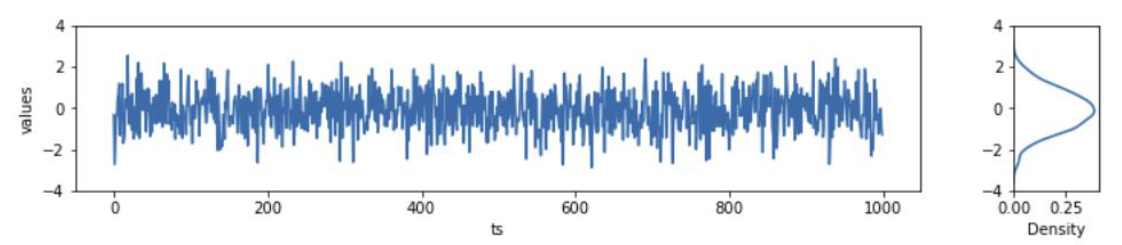
\includegraphics[width=0.8\textwidth]{figures/white_noise.png}
    \caption{White noise}
    \label{fig:white_noise}
\end{figure}

Formally: Let $\{X_t\}$ be a stochastic process and let $F_X(t_{1+ \tau}, ..., t_{k+ \tau})$
represent the cumulative distribution function of the unconditional (i.e., with no 
reference to any particular starting value) joint distribution of $\{X_t\}$ at times
$t_1 + \tau, ..., t_k + \tau$. Then, $\{X_t\}$ is said to be \textbf{strictly 
stationary}, \textbf{strongly stationary} or \textbf{strict-sense stationary}
if, for all $k$ and all $\tau$:

\begin{equation}
    F_X(t_1, ..., t_k) = F_X(t_{1 + \tau}, ..., t_{k + \tau})
\end{equation}



\section{Decomposition and detrending}

Stationarity is generally a \textbf{good property} for a time series to have, as it
makes it easier to model and predict. However, very few time series in the real world
are actually stationary. Normally, a time series includes:
\begin{itemize}
    \item a long-term trend (including aperiodic cycles).
    \item one or more seasonal patterns.
\end{itemize}

The question is: can we try to remove what causes non-stationarity? Yes, 
by \textbf{time series decomposition}.\\

\textbf{Time series decomposition} is a mathematical procedure which transforms a
time series into multiple different time series, each representing a different
component of the original one. Generally, we want to decompose a time series into
three components:
\begin{itemize}
    \item \textbf{Trend}: the long-term progression of the series.
    \item \textbf{Seasonality}: the repeating short-term cycle in the series.
    \item \textbf{Residuals}: the random noise left after the trend and seasonality
    have been removed. Hopefully, this is a stationary time series.
\end{itemize}

\begin{figure}[H]
    \centering
    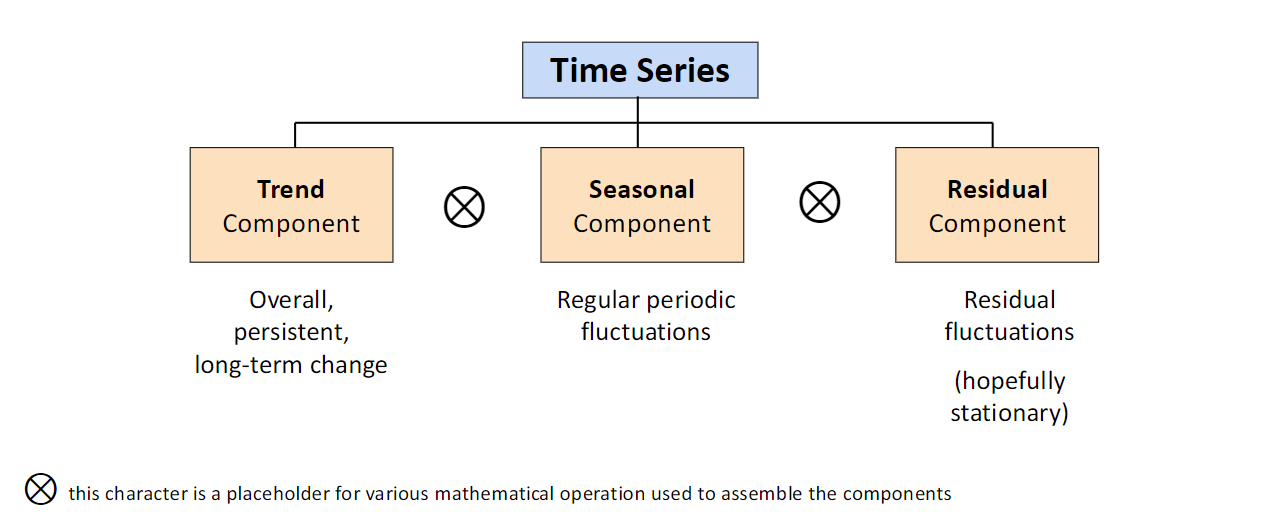
\includegraphics[width=0.9\textwidth]{figures/time_series_decomp.png}
    \caption{Time series decomposition}
    \label{fig:decomposition}
\end{figure}

\subsection{Additive and multiplicative decomposition}

We have two main methods to decompose a time series:
\begin{itemize}
    \item \textbf{Additive decomposition}: 
    $$X_t = m_t + s_t + Y_t$$

    \item \textbf{Multiplicative decomposition}:
    $$X_t = m_t \cdot s_t \cdot Y_t$$
\end{itemize}

where $X_t$ is the original time series, $m_t$ is the trend component, $s_t$ is the
seasonal component, and $Y_t$ is the residual component.\\

Which one is better? Let us see a decomposition example:

\begin{figure}[H]
    \centering
    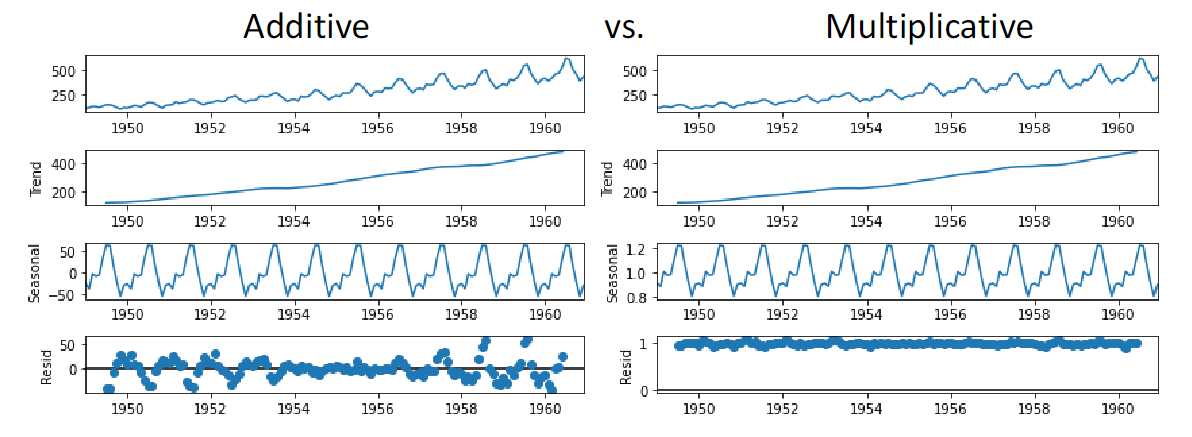
\includegraphics[width=0.9\textwidth]{figures/add_vs_mult_decomp.png}
    \caption{Additive vs multiplicative decomposition}
    \label{fig:add_vs_mult}
\end{figure}

In this case, the \textbf{multiplicative decomposition} is better because, in the
end, we obtain a residual that is more stationary than the one obtained with the
additive decomposition, which still shows some seasonality.\\

In general, we choose between additive and multiplicative decomposition based on
the following criteria:

\begin{itemize}
    \item \textbf{Additive} decomposition: it is useful when the seasonal pattern
    is relatively independent of the trend. E.g., when the seasonal variation is
    constant over time.

    \item \textbf{Multiplicative} decomposition: it is useful when the seasonal
    pattern is correlated with the trend. E.g., when it increases overtime as the
    trend increases.
\end{itemize}

Now, let us see how can we determine these decompositions. We have two main simplified
time series models, based on how many components we want to include in the decomposition:

\begin{itemize}
    \item \textbf{Non-seasonal} decomposition model with \textbf{trend}.
    \item Decomposition model with \textbf{trend} and \textbf{seasonality}.
\end{itemize}

Notice that these methods are additive decompositions. We can obtain the multiplicative
decomposition by taking the logarithm of the time series and then applying the additive
decomposition:

$$\log(X_t) = \log(m_t) + \log(s_t) + \log(Y_t)$$
$$\Rightarrow X_t = m_t \cdot s_t \cdot Y_t$$

\subsection{Non-seasonal decomposition model with trend}

This model only considers the trend component. There are two basic methods for 
estimating and removing the trend from a time series:

\begin{enumerate}
    \item \textbf{Trend elmimination by differencing}
    \item \textbf{Trend estimation by model fitting and removal}
\end{enumerate}

\subsubsection{Trend elimination by differencing}

Differencing of a time series $\{X_t\}$ in discrete time $t$ is the transformation
of the series to a new time series $\{D_t\}$, where the values are the differences
between consecutive observations:
$$d_t = x_t - x_{t-1}$$

If a trend is linear, differencing once is sufficient to remove it. If instead 
of a linear trend, we have a quadratic trend, we need to difference the series twice.
More generally, if a trend can be model with a polynomial of degree $n$, then we need
to difference the series $n$ times.

\begin{figure}[H]
    \centering
    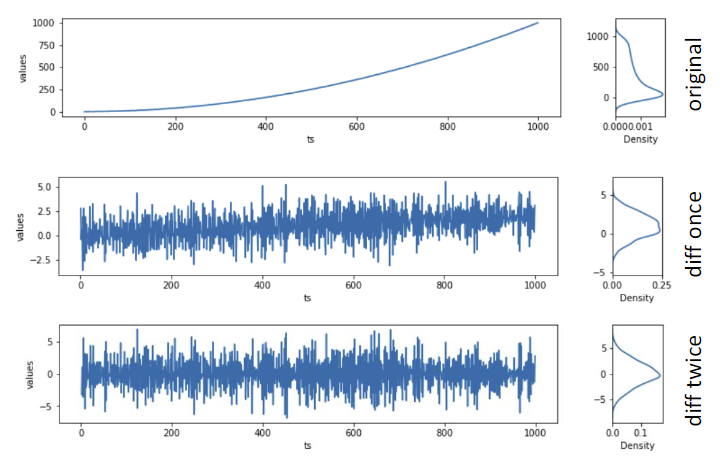
\includegraphics[width=0.6\textwidth]{figures/trend_by_diff.png}
    \caption{Removing a quadratic trend by differentiation}
    \label{fig:trend_by_diff}
\end{figure}

\subsubsection{Trend estimation by model fitting and removal}

In this method, we fit a model to the time series and then remove the model from the
series. The most common models are:
\begin{itemize}
    \item \textbf{Linear regression}: we fit a linear model to the time series and
    then subtract the model from the series.
    \item \textbf{Polynomial regression}: we fit a polynomial model to the time series
    and then subtract the model from the series.
\end{itemize}

\subsubsection{Combine the methods}

We can combine the previous tow methods, to better remove any trends from the time
series. We can do as follows:
\begin{enumerate}
    \item Differentiate the time series.
    \item Observe if the series still show a trend.
    \item If there is still a trend, detrend by fitting a regresion model (linear or
    polynomic, depending on the observed trend).
\end{enumerate}

\subsection{Decomposition model with trend and seasonality}

This method also includes a seasonal component in the decomposition. There are
3 basic methods for estimating and removing the trend and seasonality:

\begin{enumerate}
    \item \textbf{Differencing:} we differentiate one or more times to remove the
    trend. Then we perform a "seasonal differencing".

    \item \textbf{Filtering:} we estimate and remove the trend by using a "centered"
    moving average. Then we estimate and remove the seasonal component using periodic
    averages.

    \item \textbf{Joint-fit method:} fitting a combined polynomial and dynamic harmonic
    regression.
\end{enumerate}

\subsubsection{Seasonal differencing}

Seasonal differencing of a time series $\{X_t\}$ in discrete time $t$ given the
seasonality's period $d$ is the transformation of the series into a new time series
$\{S_t\}$ where the values are the differences between the value of $\{X_t\}$ at time
$t$ and the value of $\{X_t\}$ a period $d$ before:
$$s_t = x_t - x_{t-d}$$

\begin{figure}[H]
    \centering
    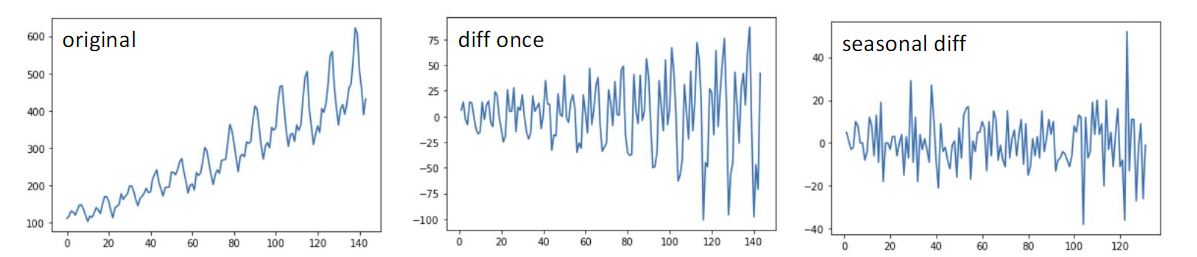
\includegraphics[width=0.9\textwidth]{figures/seasonal_diff.png}
    \caption{Seasonal differentiation of a time series}
    \label{fig:season_diff}
\end{figure}

\subsubsection{Filtering: centered moving and periodic averages}

Given the seasonality period $d$:
\begin{itemize}
    \item If $d$ is even, the "centered" moving average is defined as:
    $$\hat{m}_t = (0.5 x_{t-d} + x_{t-d+1} + ... + x_{t+d - 1} + 0.5 x_{t+d}) / d$$

    \item If $d$ is odd, then it is defined as:
    $$\hat{m}_t = (x_{t-d} + x_{t-d+1} + ... + x_{t+d - 1} + x_{t+d}) / d$$
\end{itemize}

Note that there are no values for either the first $d$ or the last $d$ points, 
because we do not have enough observations on either side to define the moving 
average for those values of $t$. Also, note that the "centered" moving average
is different from the "normal" moving average.

\begin{figure}[H]
    \centering
    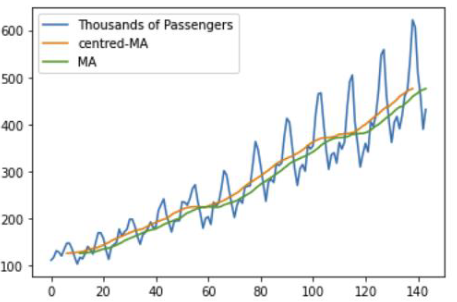
\includegraphics[width=0.55\textwidth]{figures/centered_MA.png}
    \caption{Centered moving average example}
    \label{fig:centered_MA}
\end{figure}

Now, we need to estimate the seasonal component. For that, we use \textbf{periodic
averages}:

\begin{enumerate}
    \item Divide the detrended value in seasons of length $d$. 
    \item Compute the seasonal component values $w_k$ by averaging each of the $d$
    points of the season $k = 1, ..., d$.
    \item Compute the adjusted seasonal component values $s_k$ to ensure that they
    add to zero:
    $$\hat{s}_k = w_k - d^{-1} \sum_{j=1}^d w_j, \quad k = 1, ..., d$$

    \item String together the adjusted seasonal component values in a sequence.
    \item Replace the sequence for each season.
\end{enumerate}

\begin{figure}[H]
    \centering
    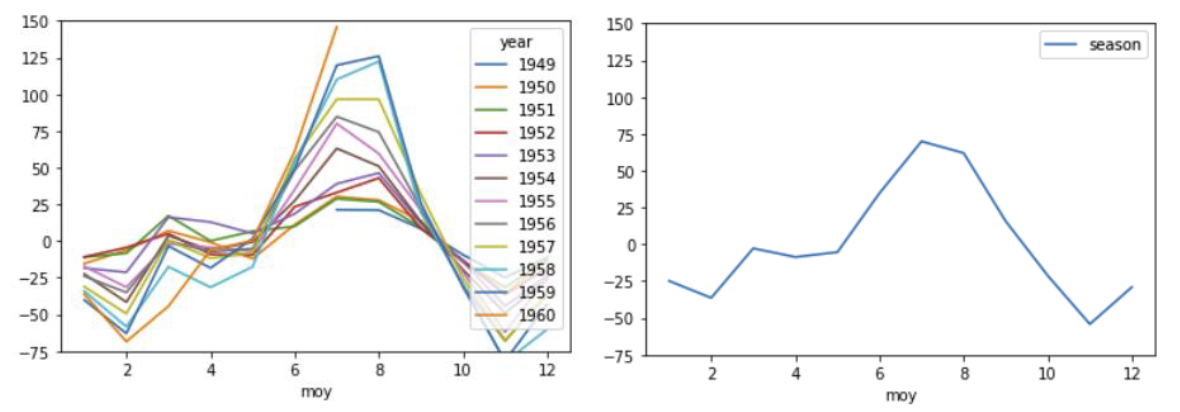
\includegraphics[width=0.9\textwidth]{figures/season_extraction.png}
    \caption{Periodic averages example}
    \label{fig:periodic_avg}
\end{figure}

\subsubsection{Joint-fit method}

This method is based on fitting a combined polynomial and dynamic harmonic regression
to estimate and then remove the trend and seasonal components simultaneously. 
The method is as follows:
$$X_t = m_t + s_t + Y_t =$$
$$=(\beta_0 +\beta_1 t + \beta_2 t^2) + \left[ \sum_{j=1}^k (\alpha_j \cos(\lambda_j t) + \gamma_j \sin(\lambda_j t)) \right] + Y_t$$

where $\beta_0, \beta_1, \beta_2$ are the coefficients of the polynomial regression
model, and $\alpha_j, \gamma_j, \lambda_j$ are the coefficients of the harmonic
regression model.\\

The following diagram represents the anatomy of the harmonic function:

\begin{figure}[H]
    \centering
    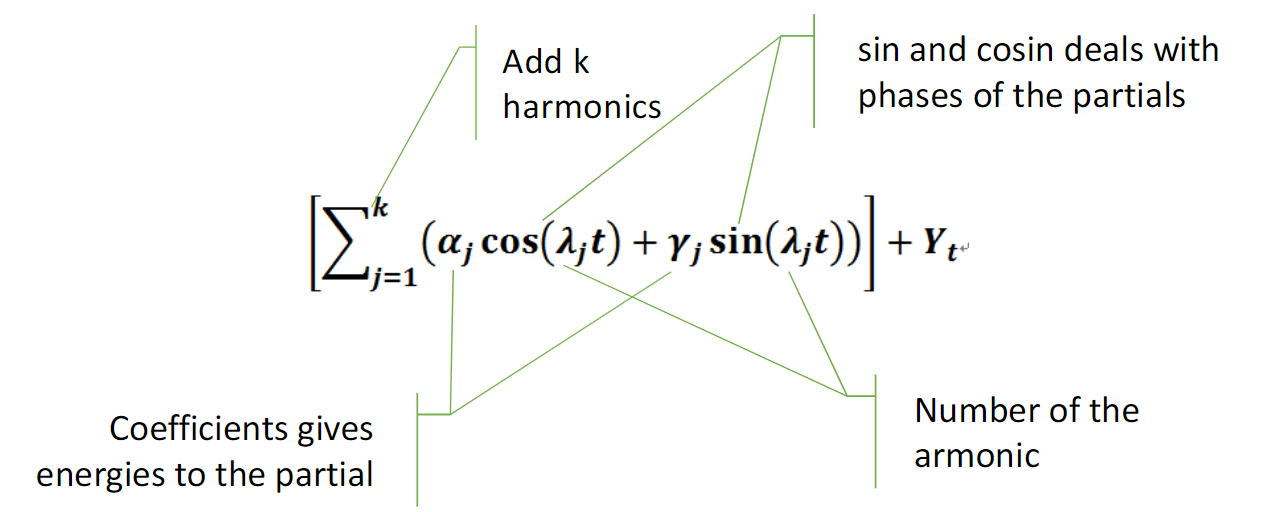
\includegraphics[width=0.85\textwidth]{figures/harmonic_function.png}
    \caption{Anatomy of the harmonic function}
    \label{fig:harmonic}
\end{figure}


\section{Forecasting baselines}

Once we have decomposed the time series into its components, we can use the residuals
to forecast the future values of the series, assuming that the residuals are stationary.\\

How far can we predict?
\begin{itemize}
    \item \textbf{Short-term forecasting}: a one-step-ahear is a forecast of the next
    observation only.
    \item \textbf{Medium and long-term forecasting}: a multi-step-ahead forecast is
    a forecast of the next $n$ observations.
\end{itemize}

What can we predict?
\begin{itemize}
    \item \textbf{Trend:} we can predict the long-term progression of the series trend.
    \item \textbf{Seasonality:} we can predict in medium-term, we don't have the certainty
    that the seasonality will repeat identically in the future.
    \item \textbf{Residuals:} we can predict the random noise left after the trend and
    seasonality have been removed. This is the most difficult component to predict, and
    we can predict it only in the short-term.
\end{itemize}

The overall forecasting process is based on decomposing the time series 
$\{X_t\}$ into its components, then we predict the residuals, add the seasonality
component and finally add the trend component based on the fitting models.

\begin{figure}[H]
    \centering
    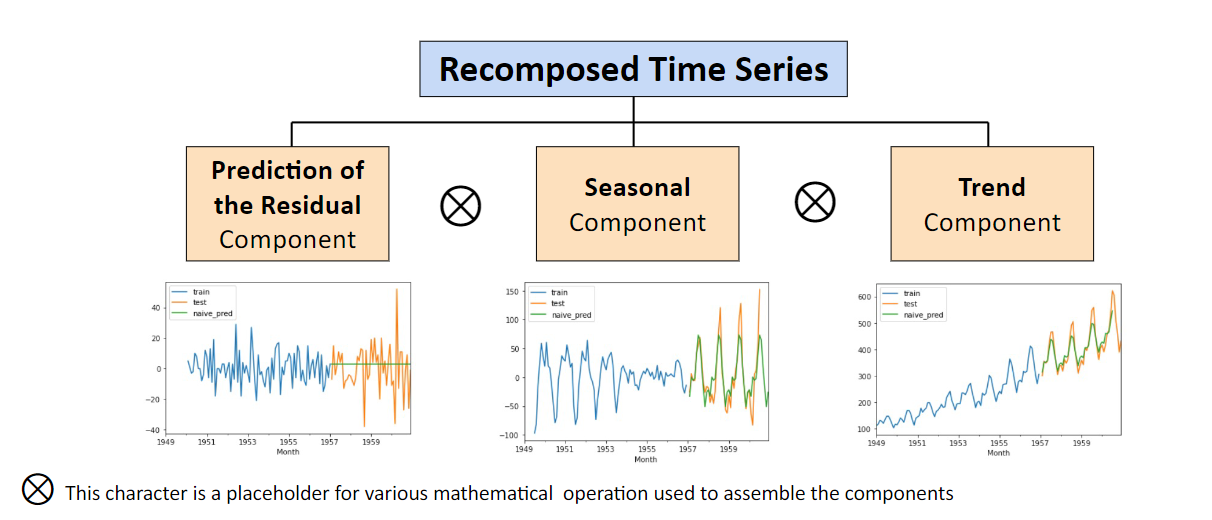
\includegraphics[width=0.9\textwidth]{figures/recompose_time_series.png}
    \caption{Recomposition of the time series}
    \label{fig:recompose}
\end{figure}

\subsection{Error metrics}

To evaluate the quality of the forecast, we need to compare the forecasted values
with the actual values on the test set. The most common error metrics are:

\begin{itemize}
    \item \textbf{Mean Absolute Error (MAE)}:
    $$MAE = \frac{1}{n} \sum_{i=1}^n |y_i - \hat{y}_i|$$

    \item \textbf{Mean Absolute Percentage Error (MAPE)}:
    $$MAPE = \frac{100}{n} \sum_{i=1}^n \left| \frac{y_i - \hat{y}_i}{y_i} \right|$$

    \item \textbf{Mean Squared Error (MSE)}:
    $$MSE = \frac{1}{n} \sum_{i=1}^n (y_i - \hat{y}_i)^2$$

    \item \textbf{Root Mean Squared Error (RMSE)}:
    $$RMSE = \sqrt{MSE} = \sqrt{\frac{1}{n} \sum_{i=1}^n (y_i - \hat{y}_i)^2}$$
\end{itemize}

How do we choose which error metric to use? It depends on the context of the problem.
The following table shows the benefits and limitations of each error metric:

\begin{figure}[H]
    \centering
    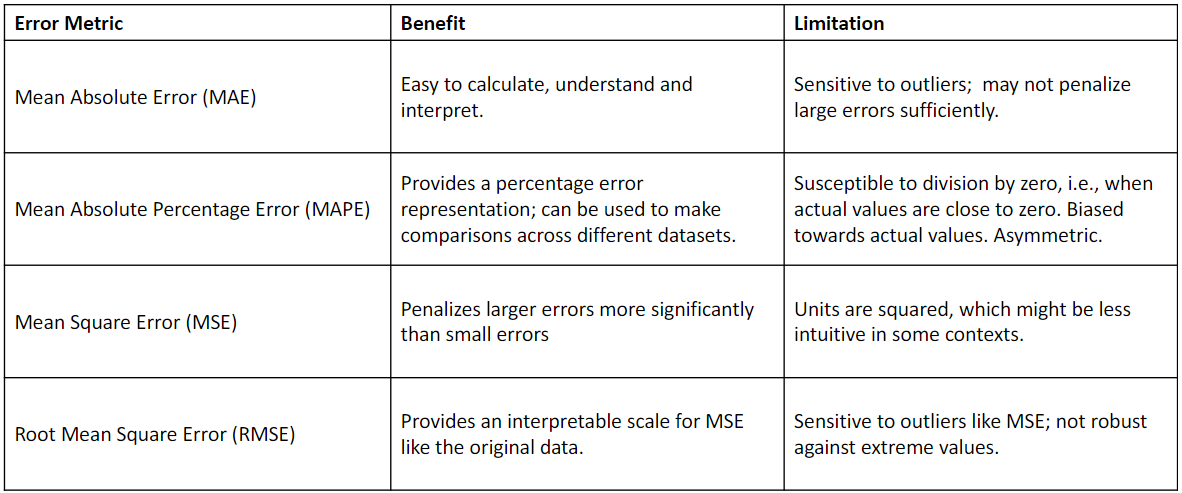
\includegraphics[width=0.9\textwidth]{figures/error_metrics.png}
    \caption{Error metrics}
    \label{fig:error_metrics}
\end{figure}

\subsection{Basic forecasting methods}

The residuals are the random noise left after the trend and seasonality have been
removed. We can predict the residuals using the following baseline methods:

\begin{itemize}
    \item \textbf{Naive approach:} The only important information is the last value
    of the residuals. We can predict the residuals as the last value of the residuals
    in the training set:
    $$\hat{y}_{t+1} = y_t$$

    \item \textbf{Mean approach:} We can predict the residuals as the mean of the residuals
    in the training set:
    $$\hat{y}_{t+1} = \frac{1}{n} \sum_{i=1}^n y_i$$
\end{itemize}

We also have a more sophisticated method to predict the residuals, which is the
\textbf{last-k average} approach. This method appears to be in the middle between
the naive and mean approaches. The method is as follows:
$$\hat{y}_{t+1} = \frac{1}{k} \sum_{i=1}^k y_{t-i}$$

The problem with this method is that we need to choose the value of $k$, which is
a hyperparameter. It is hard to set a value that clearly separates the data to
"forget" and the data to use for the prediction.\\

We ask the question: is there a way to consider all the data in the training set
while still introducing a "forgetting" mechanism? Yes, we can use the \textbf{exponential
smoothing} method.

\subsection{Exponential smoothing}

\textbf{Exponential smoothing} is a \textbf{stationary time series} forecasting method for univariate 
data. It is a simple yet effective method for forecasting. The method is based on the idea
of weighting the most recent observations more heavily than the older observations.\\

The method is as follows:
$$\hat{y}_{t+1} = \alpha y_t + (1 - \alpha) \hat{y}_t$$

where $\alpha$ is the smoothing factor, which is a value between 0 and 1. The value
of $\alpha$ determines the weight of the most recent observation. The closer $\alpha$
is to 1, the more weight is given to the most recent observation. The closer $\alpha$
is to 0, the more weight is given to the previous forecast.\\

Often, it is easier to set $\alpha$ as the number of points (span) with a 
considerable impact on the forecast:
$$\alpha = \frac{2}{span + 1}$$

Notice that this is a \textbf{streaming algorithm}, which means that we can update
the forecast only as fast as new observations become available. This is because
the forecast at time $t+1$ depends on the forecast at time $t$ and the true observation
at time $t$. \\

Also, if we rearrange the formula, we get:
$$\hat{y}_{t+1} = \alpha y_t + (1 - \alpha) \hat{y}_t = \hat{y}_t + \alpha(y_t - \hat{y}_t)$$

This shows that the next prediction is the sum of the current prediction and a correction
term. The correction term is propotional (with factor $\alpha$) to the current error, 
which is the difference between the current observation and the current prediction.\\

Also notice that we need a starting value for the forecast, then we have:
$$\hat{y}_1 = \ell_0$$
$$\hat{y}_{t} = \alpha y_{t-1} + (1 - \alpha) \hat{y}_{t-1}$$

where $\ell_0$ is the starting value of the forecast. We can set $\ell_0$ as the
first value of the residuals in the training set.\\

What about directly forecasting a time series with trend and seasonality? We can
extend the exponential smoothing method to include only the trend component 
or both the trend and seasonal components:
\begin{itemize}
    \item Residual + trend: \textbf{Holt's linear trend method}, also known as
    \textbf{double exponential smoothing}.
    \item Residual + trend + seasonality: \textbf{Holt-Winters' method}, also known
    as \textbf{triple exponential smoothing}.
\end{itemize}

\subsection{Double exponential smoothing: Holt's linear method}

\textbf{Holt's linear method} is an extension of the exponential smoothing method
tha \textbf{adds support for trends} using an additional smoothing factor $\beta$
to control the decay of the influence of the change in trend.\\

This method supports trends that change in different ways:
\begin{itemize}
    \item \textbf{Additive}, when the trend is linear:
    \begin{align*}
        \text{Forecast equation: } &\hat{y}_{t+h} = \ell_t + h \cdot b_t\\
        \text{Level equation: } &\ell_t = \alpha y_t + (1 - \alpha)(\ell_{t-1} + b_{t-1})\\
        \text{Trend equation: } &b_t = \beta(\ell_t - \ell_{t-1}) + (1 - \beta)b_{t-1}
    \end{align*}

    \item \textbf{Multiplicative}, when the trend is exponential. This only changes
    the forecast equation:
    $$\hat{y}_{t+h} = \ell_t \cdot (b_t)^h$$
\end{itemize}

Let us take a look at the anatomy of the Holt's linear method:

\begin{figure}[H]
    \centering
    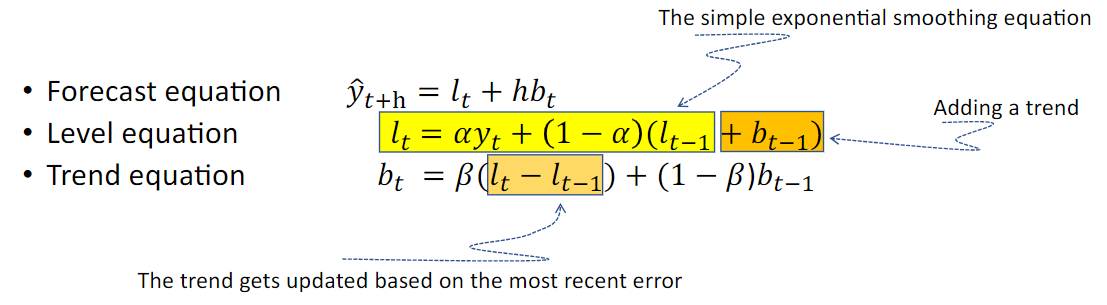
\includegraphics[width=0.9\textwidth]{figures/holt_linear.png}
    \caption{Anatomy of Holt's linear method}
    \label{fig:holt_linear}
\end{figure}

Note that the trend can vary adaptively over time. The trend smoothing factor $\beta$
is used to control the decay of the influence of the change in trend. The closer
$\beta$ is to 1, the more weight is given to the most recent trend. The closer
$\beta$ is to 0, the more weight is given to the previous trend.

\subsection{Triple exponential smoothing: Holt-Winters' method}

\textbf{Holt-Winters' method} is an extension of the Holt's linear method that
\textbf{adds support for seasonality} using an additional smoothing factor $\gamma$
to control the decay of the influence of the change in seasonality.\\

As with the trend, the seasonality may be modelled as an \textbf{additive or 
multiplicative} process for a linear or exponential change in the seasonality.\\

The equations for the additive method, for a time series with seasonality of period
$d$ are:
\begin{align*}
    \text{Forecast equation: } &\hat{y}_{t+h} = \ell_t + h \cdot b_t + s_{t-d+h}\\
    \text{Level equation: } &\ell_t = \alpha(y_t - s_{t-d}) + (1 - \alpha)(\ell_{t-1} + b_{t-1})\\
    \text{Trend equation: } &b_t = \beta(\ell_t - \ell_{t-1}) + (1 - \beta)b_{t-1}\\
    \text{Seasonal equation: } &s_t = \gamma(y_t - \ell_{t-1} - b_{t-1}) + (1 - \gamma)s_{t-d}
\end{align*}

Let us take a look at the anatomy of the Holt-Winters' method:

\begin{figure}[H]
    \centering
    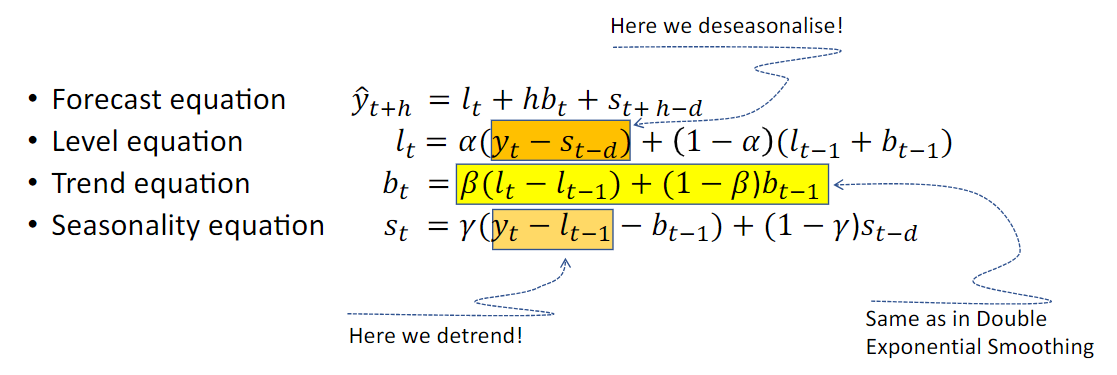
\includegraphics[width=0.9\textwidth]{figures/holt_winters.png}
    \caption{Anatomy of Holt-Winters' method}
    \label{fig:holt_winters}
\end{figure}

Note that both the trend and seasonality can vary adaptively over time. The trend
smoothing level $\beta$ and the seasonality smoothing level $\gamma$ are used to
control the speed of adjusting the trend and seasonality, respectively. The only 
fixed parameter is the seasonality period $d$.

\section{Second foundational concept: Temporal dependence}

The second foundational concept in time series analysis is \textbf{temporal dependence}.
Temporal dependence is the idea that the value of a time series at time $t$ is
dependent on the values of the time series at previous times.\\

To understand temporal dependence, we need to introduce the following concepts:
\begin{itemize}
    \item \textbf{Correlation}
    \item \textbf{Autocorrelation}
    \item \textbf{Partial autocorrelation}
\end{itemize}

\subsection{Correlation}

\textbf{Correlation} is a measure of the strength and direction of a linear relationship
between two variables. In other words, measures the degree to which two variables
$X_1$ and $X_2$ move in coordination with each other.\\

The correlation coefficient is a value between -1 and 1. The closer the value is to
1, the stronger the positive correlation, meaning that the two variables move in the
same direction. The closer the value is to -1, the stronger the negative correlation,
meaning that the two variables move in opposite directions. A value of 0 indicates
no correlation.

\begin{figure}[H]
    \centering
    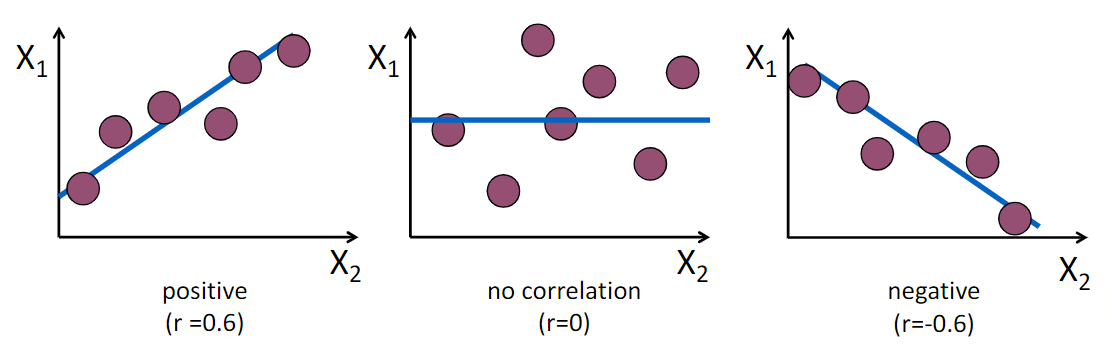
\includegraphics[width=0.9\textwidth]{figures/correlation.png}
    \caption{Correlation examples}
    \label{fig:correlation}
\end{figure}

The correlation coefficient is defined as:
$$\rho_{X_1, X_2} = Corr(X_1, X_2) = \frac{Cov(X_1, X_2)}{\sigma_{X_1} \sigma_{X_2}}$$

where $Cov(X_1, X_2)$ is the covariance between $X_1$ and $X_2$, and $\sigma_{X_1}$
and $\sigma_{X_2}$ are the standard deviations of $X_1$ and $X_2$, respectively.

\subsection{Autocorrelation}

\textbf{Autocorrelation} is a measure of the strength and direction of a linear relationship
between a time series and a lagged version of itself. In other words, it measures the
degree to which the value of a time series at time $t$ is dependent on the value of the
time series at time $t - k$, where $k$ is the lag.\\

The \textbf{autocorrelation function (ACF)} is a plot of the autocorrelation of a time series
against the lag. The ACF is used to identify the presence of temporal dependence in
a time series.

\begin{figure}[H]
    \centering
    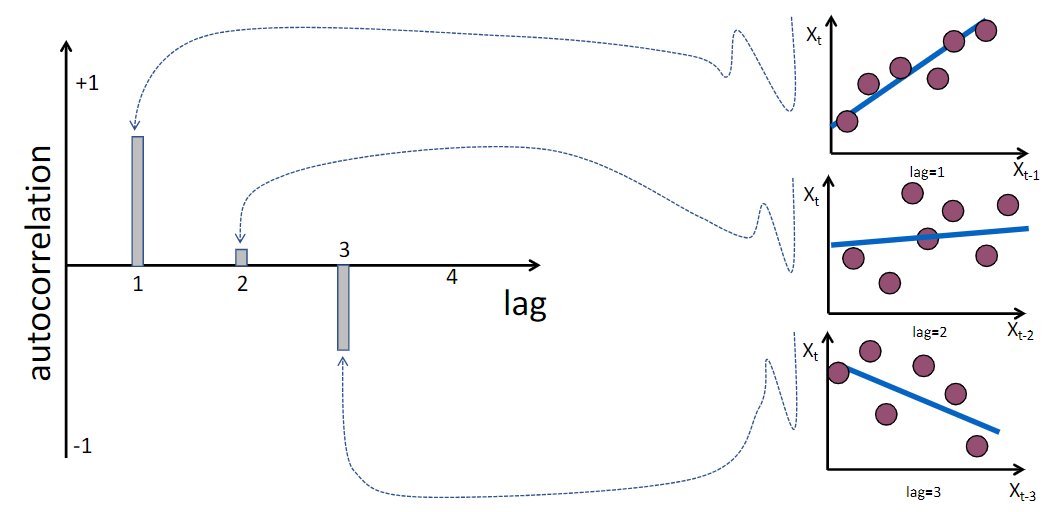
\includegraphics[width=0.85\textwidth]{figures/acf.png}
    \caption{Autocorrelation function}
    \label{fig:acf}
\end{figure}

The autocorrelation coefficient at lag $k$ is defined as the correlation between the
time series and a lagged version of itself:
$$\rho_k = Corr(X_t, X_{t-k})$$

Let us see an example of the autocorrelation function, for a time series representing
the number of passengers on an airline flight:

\begin{figure}[H]
    \centering
    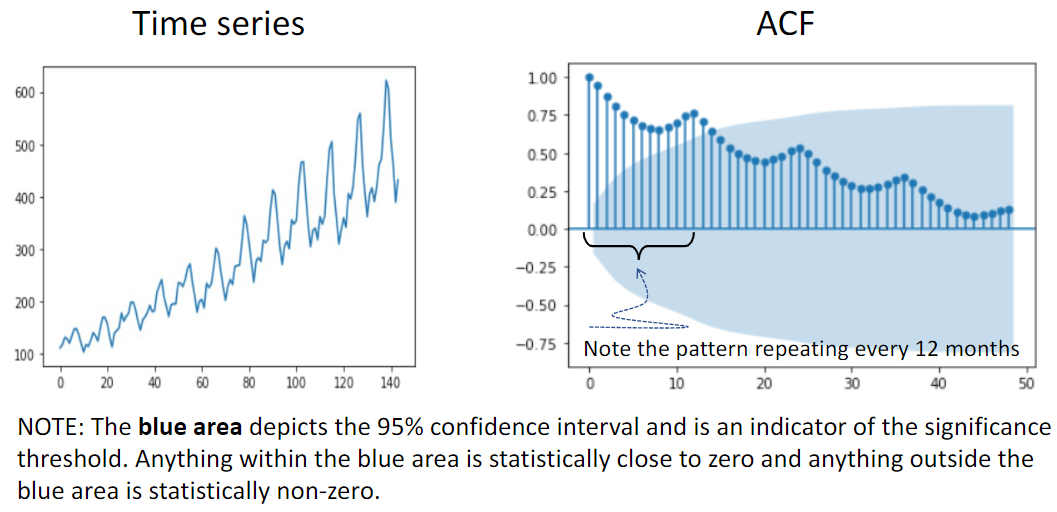
\includegraphics[width=0.95\textwidth]{figures/acf_example.png}
    \caption{Autocorrelation function example}
    \label{fig:acf_example}
\end{figure}

This example depicts the presence of a seasonality with a period of 12 months. The
autocorrelation function shows a peak at lag 12, which indicates that the number of
passengers in a given month is correlated with the number of passengers 12 months
earlier.

\subsection{Partial autocorrelation}

\textbf{Partial autocorrelation} is a measure of the strength and direction of a linear
relationship between a time series and a lagged version of itself, after accounting for
the effect of other lags. In other words, it measures the degree to which the value of
a time series at time $t$ is dependent on the value of the time series at time $t - k$,
after removing the effect of the intermediate lags $t - 1, t - 2, ..., t - k + 1$.\\

To calculate the partial autocorrelation coefficient at lag $k$, we need to fit a linear
regression model to the time series using the intermediate lags as predictors. The
partial autocorrelation coefficient is the coefficient of the lag $k$ in the regression
model. In other words, if we compute the OLS regression of $X_t$ on $X_{t-1}, X_{t-2}, ...,
X_{t--k}$:

$$X_t = \beta_0 + \beta_1 X_{t-1} + \beta_2 X_{t-2} + ... + \beta_k X_{t-k} + \epsilon_t$$

then the partial autocorrelation coefficient at lag $k$ is $\rho_k = \beta_k$.\\

The \textbf{partial autocorrelation function (PACF)} is a plot of the partial autocorrelation
of a time series against the lag. The PACF is used to identify the presence of temporal
dependence in a time series.

\begin{figure}[H]
    \centering
    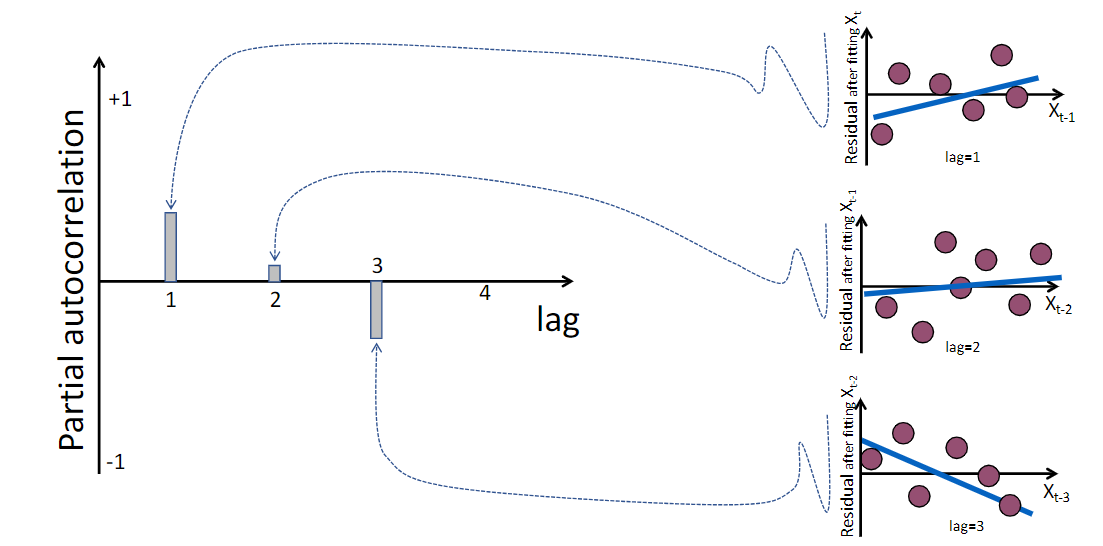
\includegraphics[width=0.85\textwidth]{figures/pacf.png}
    \caption{Partial autocorrelation function}
    \label{fig:pacf}
\end{figure}

Note that the PACF at lag $k = 1$ does not consider any intermediate observations. It
is essentially the correlation between observations $y_t$ and $y_{t-1}$ while ignoring
the effect of any other lags (there are no intermediate lags). So the PACF at lag $k = 1$
is the same as the ACF at lag $k = 1$:
$$PACF(1) = ACF(1) = Corr(y_t, y_{t-1})$$

\section{ARMA models}

\textbf{ARMA} stands for \textbf{Auto Regressive Moving Average} models. 
ARMA models are used to model and forecast \textbf{stationary time series}. An ARMA
model of order $(p, q)$ is the sum of:
\begin{itemize}
    \item an \textbf{Auto Regressive (AR) model} of order $p$
    \item a \textbf{Moving Average (MA) model} of order $q$ 
\end{itemize}

\begin{figure}[H]
    \centering
    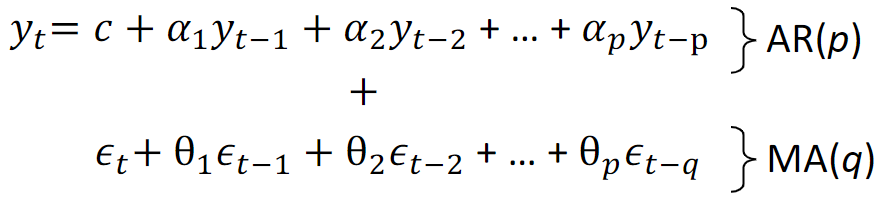
\includegraphics[width=0.6\textwidth]{figures/arma_eq.png}
    \caption{ARMA model equation}
    \label{fig:arma_eq}
\end{figure}

\subsection{Auto Regressive (AR) model}

An \textbf{Auto Regressive (AR) model} of order $p$, denoted as $AR(p)$, models a 
time series so that the current value of a time series is a linear combination of
the \textbf{past $p$ values of the time series} plus a white noise term $\epsilon_t$:

\begin{equation}
    y_t = c + \alpha_1 y_{t-1} + \alpha_2 y_{t-2} + ... + \alpha_p y_{t-p} + \epsilon_t = c + \sum_{i=1}^p \alpha_i y_{t-i} + \epsilon_t
\end{equation}

where $c$ is a constant, $\alpha_1, ..., \alpha_p$ are the coefficients of the model,
and $\epsilon_t$ is the white noise term. Notice that, in some way it is similar to 
the exponential smoothing method, but the AR model only uses $p$ values and the
weights $\alpha_i$ do not decay exponentially.\\

This method can improve the forcast with an horizon smaller than $p$ (short-term).

\begin{figure}[H]
    \centering
    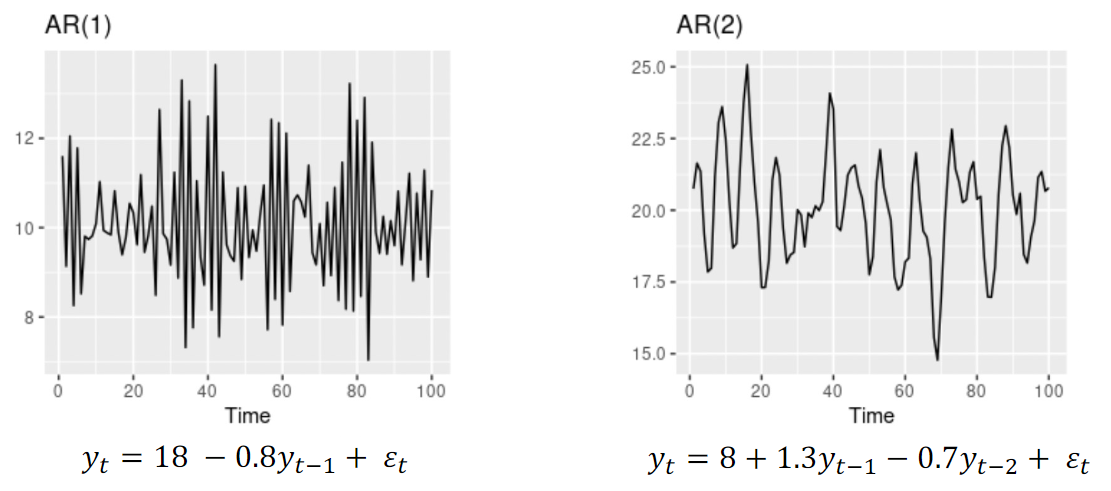
\includegraphics[width=0.9\textwidth]{figures/ar_model.png}
    \caption{Auto Regressive models example}
    \label{fig:ar_model}
\end{figure}

Let us see some special $AR(1)$ models:
\begin{itemize}
    \item When $c = \alpha_1 = 0$, $AR(1)$ is equivalent to a white noise model.
    \item When $c = 0$ and $\alpha = 1$, $AR(1)$ is equivalent to a random walk model.
    \item When $c \neq 0$ and $\alpha = 1$, $AR(1)$ is equivalent to a random walk with drift model.
    \item When $c = 0$ and $\alpha < 1$, $AR(1)$ tends to oscillate between positive and
    negative values.
\end{itemize}

\subsection{Moving Average (MA) model}

A \textbf{Moving Average (MA) model} of order $q$, denoted as $MA(q)$, models the 
residual of a time series using \textbf{regression of past q estimation errors}:

\begin{equation}
    y_t = c + \epsilon_t + \theta_1 \epsilon_{t-1} + \theta_2 \epsilon_{t-2} + ... + \theta_q \epsilon_{t-q} = c + \sum_{i=1}^q \theta_i \epsilon_{t-i} + \epsilon_t
\end{equation}

where $c$ is a constant, $\theta_1, ..., \theta_q$ are the coefficients of the model,
and $\epsilon_t$ is the white noise term. Note that this model works on estimation errors,
and it is different from the moving average of the time series.

\begin{figure}[H]
    \centering
    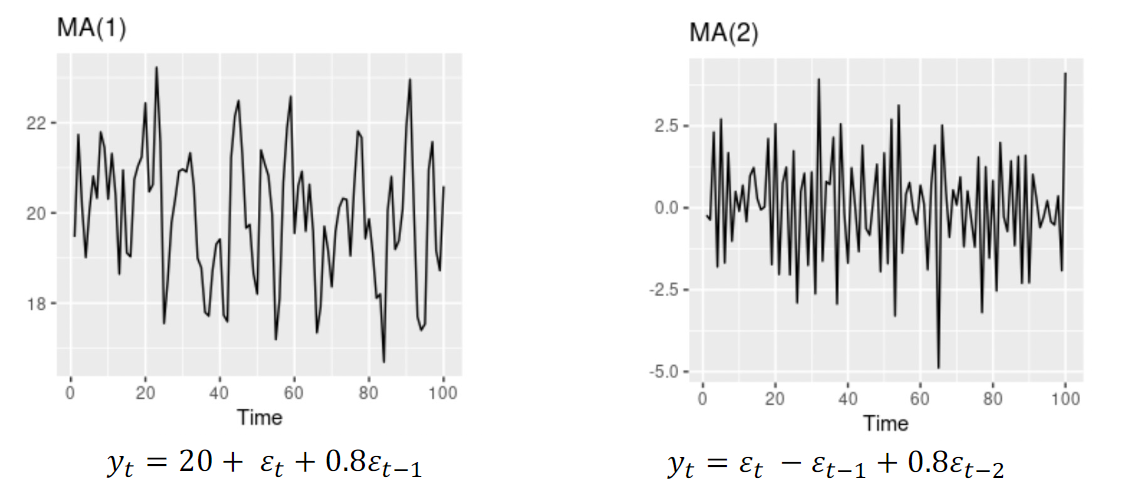
\includegraphics[width=0.9\textwidth]{figures/ma_model.png}
    \caption{Moving Average models example}
    \label{fig:ma_model}
\end{figure}

\subsubsection{From $AR(p)$ to $MA(\infty)$}

It is possible to write any \textbf{stationary} $AR(p)$ model as an $MA(\infty)$ model.
For example, using repeated substitution, we can demonstrate this for an $AR(1)$ model:
\begin{align*}
    y_t &= \alpha_1 y_{t-1} + \epsilon_t\\
    &= \alpha_1 (\alpha_1 y_{t-2} + \epsilon_{t-1}) + \epsilon_t\\
    &= \alpha_1^2 y_{t-2} + \alpha_1 \epsilon_{t-1} + \epsilon_t\\
    &= \alpha_1^3 y_{t-3} + \alpha_1^2 \epsilon_{t-2} + \alpha_1 \epsilon_{t-1} + \epsilon_t\\
    &...
\end{align*}

Provided $-1 < \alpha_1 < 1$, the value of $\alpha_1^k$ will get smaller as $k$ gets
larger. So eventually, we obtain the above equation equal to an $MA(\infty)$ model.

\subsection{ARIMA model: ARMA + differencing}

\textbf{ARIMA} stands for \textbf{Auto Regressive Integrated Moving Average} models.
ARIMA models are a generalization of ARMA models that include \textbf{differencing} to
make the time series stationary, by removing the trend component. Notice that this 
method \textbf{does not address the seasonality component}, so we need to remove it before
applying the ARIMA model (e.g., by seasonal differencing).\\

An ARIMA model of order $(p, d, q)$ is the sum of:
\begin{itemize}
    \item an \textbf{Auto Regressive (AR) model} of $p$ previous lagged values
    \item a \textbf{Moving Average (MA) model} of $q$ previous lagged estimation errors
\end{itemize}

\begin{figure}[H]
    \centering
    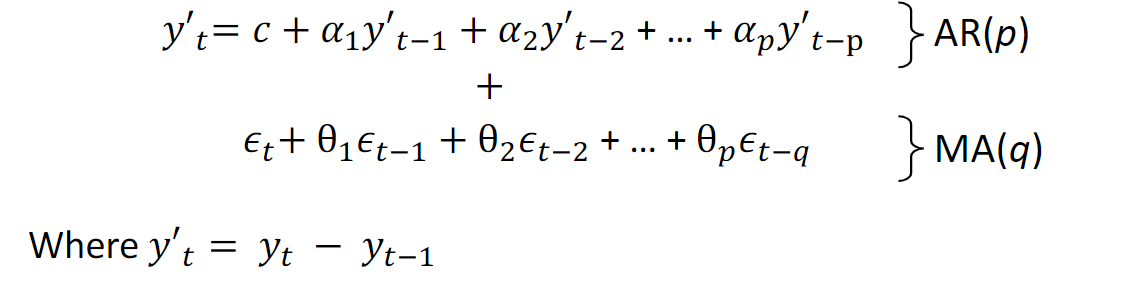
\includegraphics[width=0.6\textwidth]{figures/arima_eq.png}
    \caption{ARIMA model equation}
    \label{fig:arima_eq}
\end{figure}

Notice that the parameter $d$ is the order of differencing. The goal is
to remove the trend component of the time series. In other words, if we have a 
linear trend, we use $d = 1$ to remove it. If we have a quadratic trend, we use
$d = 2$ to remove it, and so on.\\

The biggest question is: \textbf{how do we choose the values of $p$ and $q$?} We can
use the \textbf{ACF} and \textbf{PACF} plots to determine the values of $p$ and $q$,
using the \textbf{Box-Jenkins methodology}.

\subsection{Box-Jenkins method}

The \textbf{Box-Jenkins methodology} helps us to determine the values of $p$ and $q$
for an ARIMA model, along with evaluating the model's goodness of fit. The methodology
is as follows:

\begin{enumerate}
    \item \textbf{Identification:} determine the order of differencing $d$ to make the
    time series stationary. Then, determine the values of $p$ and $q$ using the ACF
    and PACF plots.

    \item \textbf{Estimation:} fit the ARIMA model to the time series using the values
    of $p$, $d$, and $q$ determined in the identification step.

    \item \textbf{Diagnostic checking:} evaluate the goodness of fit of the ARIMA model
    using the residuals. The residuals should be white noise, meaning that they are
    uncorrelated and have constant variance.

    \item \textbf{Forecasting:} use the ARIMA model to forecast future values of the
    time series.
\end{enumerate}

This process is iterative, meaning that we may need to go back and forth between the
steps to refine the values of $p$ and $q$ and to improve the model's goodness of fit.

\subsubsection{Identification step}

The identification step is the most important step in the Box-Jenkins methodology.
The goal is to determine the values of $p$ and $q$ using the ACF and PACF plots. In
general, we use the following rules to determine the values of $p$ and $q$:

\begin{itemize}
    \item \textbf{AR model:} the ACF plot of an AR model will show a \textbf{slow decay}
    and the PACF plot will show a \textbf{sharp cutoff} after lag $p$. In this case,
    the model is ARMA$(p, 0)$ (order of AR model is $p$).

    \begin{figure}[H]
        \centering
        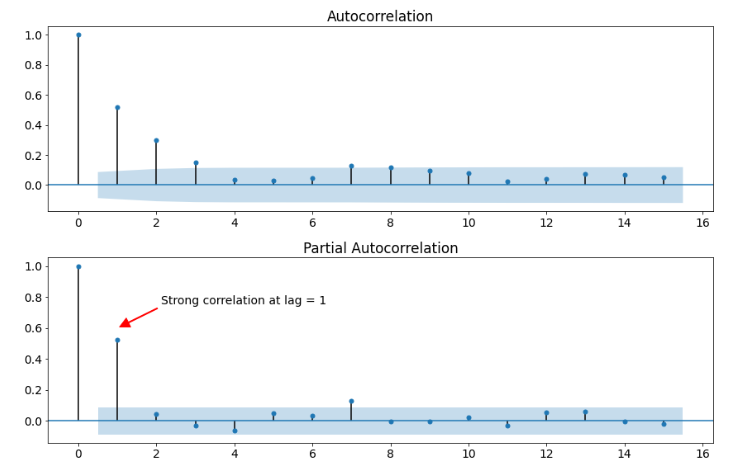
\includegraphics[width=0.6\textwidth]{figures/ARMA_1_0.png}
        \caption{Example of an ARMA$(1, 0)$ model}
        \label{fig:arma_1_0}
    \end{figure}


    \item \textbf{MA model:} the PACF plot of an MA model will show a \textbf{slow decay}
    and the ACF plot will show a \textbf{sharp cutoff} after lag $q$. In this case,
    the model is ARMA$(0, q)$ (order of MA model is $q$).

    \begin{figure}[H]
        \centering
        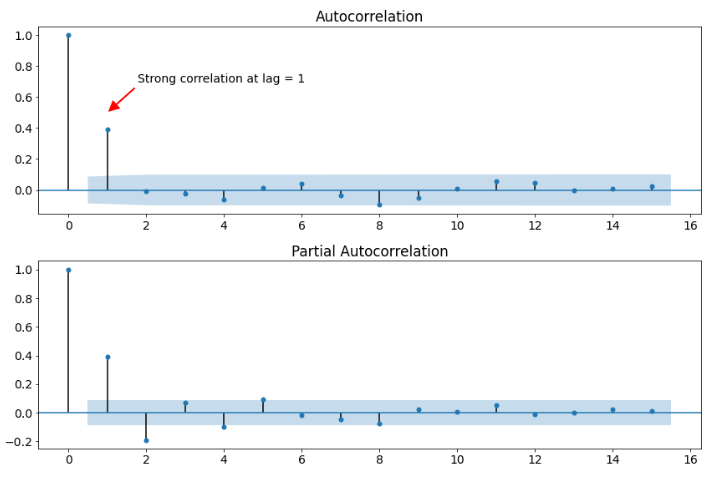
\includegraphics[width=0.6\textwidth]{figures/ARMA_0_1.png}
        \caption{Example of an ARMA$(0, 1)$ model}
        \label{fig:arma_0_1}
    \end{figure}
\end{itemize}

We can also perform what is known as \textbf{grid search} to determine the values of
$p$ and $q$. We can fit multiple ARIMA models with different values of $p$ and $q$,
and then evaluate the models using the AIC or BIC criteria. The model with the lowest
AIC or BIC value is the best model.\\

The \textbf{Akaike Information Criterion (AIC)} is a measure of the goodness of fit of
a model. The AIC is defined as:

$$AIC = -2 \log(L) + 2k$$

where $L$ is the likelihood of the model and $k$ is the number of parameters in the model.

The \textbf{Bayesian Information Criterion (BIC)} is also a measure of the goodness of fit of
a model. The BIC is defined as:

$$BIC = -2 \log(L) + k \log(n)$$

where $L$ is the likelihood of the model, $k$ is the number of parameters in the model,
and $n$ is the number of observations in the time series.

\subsubsection{Estimation step}

The estimation step is the process of fitting the ARIMA model to the time series using
the values of $p$, $d$, and $q$ determined in the identification step. The goal is to
estimate the coefficients of the model that best describe the time series. The estimation
step is done using the maximum likelihood estimation method.\\

In general, there are tools that can help us to fit the ARIMA model to the time series,
such as the \textbf{statsmodels} library in Python. We will not cover in details the
estimation step, as it is a technical process that requires knowledge of the maximum
likelihood estimation method.

\subsubsection{Diagnostic checking step}

The diagnostic checking step is the process of evaluating the goodness of fit of the
ARIMA model using the residuals. The residuals should be white noise, meaning that they
are uncorrelated and have constant variance.\\

The diagnostic checking step is done using one or more of the following tools:

\begin{itemize}
    \item \textbf{Residual plots:} plot the residuals of the ARIMA model to check for
    patterns or trends. The residuals should be randomly distributed around zero.

    \item \textbf{ACF and PACF plots of the residuals:} plot the ACF and PACF of the
    residuals to check for autocorrelation. The ACF and PACF of the residuals should
    not show any significant autocorrelation.

    \item \textbf{Ljung-Box test:} perform the Ljung-Box test on the residuals to check
    for autocorrelation. The Ljung-Box test is a statistical test that tests the null
    hypothesis that the residuals are uncorrelated. In general, if the p-value of the
    Ljung-Box test is less than 0.05, we reject the null hypothesis and conclude that
    the residuals are correlated.

    \item \textbf{Jarque-Bera test:} perform the Jarque-Bera test on the residuals to
    check for normality. The Jarque-Bera test is a statistical test that tests the null
    hypothesis that the residuals are normally distributed. In general, if the p-value
    of the Jarque-Bera test is less than 0.05, we reject the null hypothesis and conclude
    that the residuals are not normally distributed.
\end{itemize}

We also have other tools to evaluate the randomness of the residuals, depicted in the
following figure:

\begin{figure}[H]
    \centering
    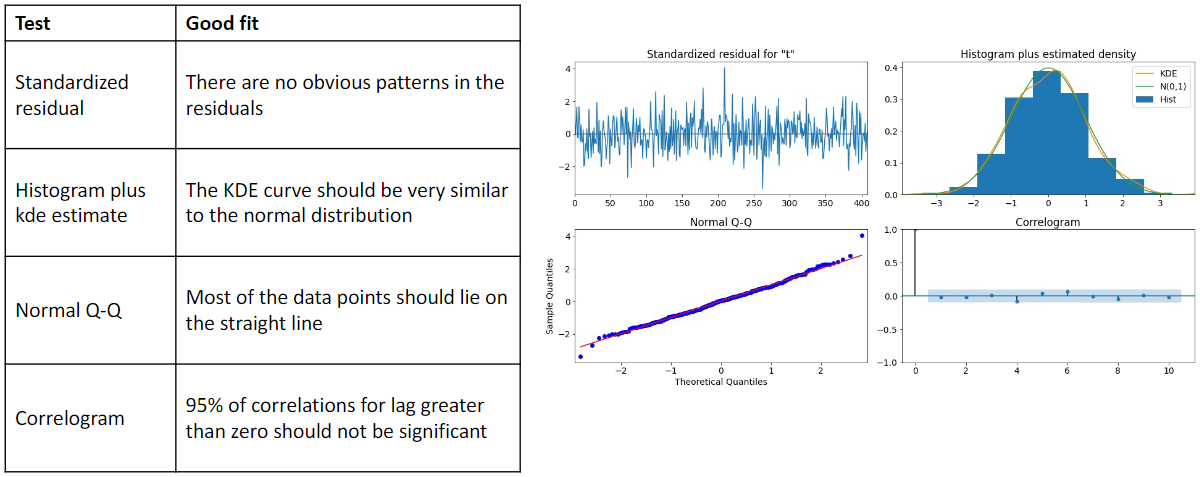
\includegraphics[width=0.95\textwidth]{figures/residuals.png}
    \caption{Residuals evaluation tools}
    \label{fig:residuals}
\end{figure}

\subsubsection{Forecasting step}

The forecasting step is the process of using the ARIMA model to forecast future values
of the time series. The ARIMA model can be used to forecast the next $n$ observations
of the time series. The forecasted values are based on the estimated coefficients of
the model and the observed values of the time series.\\

Note that, over time, errors accumulate, leading to straight line forecasts. In general, over 
the limits of order $p$ and $q$, \textbf{predictions tend to converge into a constant value}, due
to reliance on forecasted values. This is known as the \textbf{forecast horizon problem}.\\

In the end, \textbf{prolonged predictions may result in a loss of accuracy}, often manifesting
as a linear trend or stable value over time.

\subsection{Seasonal ARIMA models (SARIMA)}

\textbf{Seasonal ARIMA (SARIMA)} models are an extension of ARIMA models that include seasonal
components. Seasonal ARIMA models are used to model and forecast time series with
seasonality. A seasonal ARIMA model of order $(p, d, q)(P, D, Q)_s$ is the sum of:

\begin{itemize}
    \item an \textbf{Auto Regressive (AR) model} of order $p$ and seasonal order $P$
    \item a \textbf{Moving Average (MA) model} of order $q$ and seasonal order $Q$
    \item differencing of order $d$ and seasonal order $D$
\end{itemize}

This model is very similar to the ARIMA model, except that there is an \textbf{additional
set of autoregressive and moving average terms} to account for the seasonality (of
period $s$). The SARIMA model is defined as:

\begin{figure}[H]
    \centering
    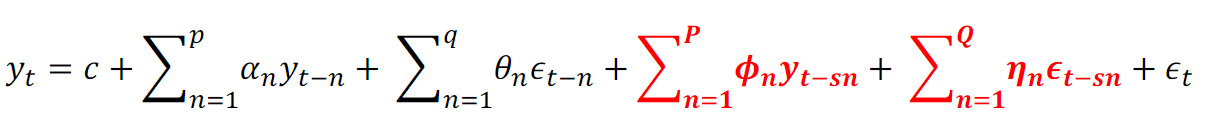
\includegraphics[width=0.9\textwidth]{figures/seasonal_arima.png}
    \caption{Seasonal ARIMA model equation}
    \label{fig:seasonal_arima_eq}
\end{figure}

\subsection{SARIMAX}

\textbf{SARIMAX} models are an extension of SARIMA models that include exogenous variables.
Exogenous variables are external variables that are not part of the time series but may
influence the time series. SARIMAX models are used to model and forecast time series with
seasonality and exogenous variables.\\

SARIMAX includes all the components of SARIMA models, but with an extension to \textbf{incorporate
$r$ exogenous variables} $X_t = (x_{1,t}, x_{2,t}, ..., x_{r,t})$. The SARIMAX model is defined as:

\begin{figure}[H]
    \centering
    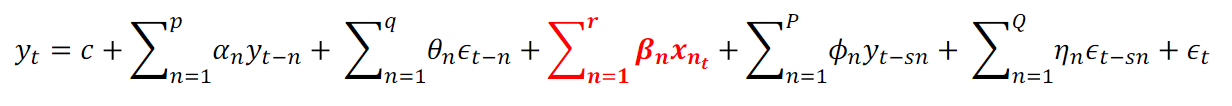
\includegraphics[width=0.95\textwidth]{figures/sarimax.png}
    \caption{SARIMAX model equation}
    \label{fig:sarimax_eq}
\end{figure}

\section{Practical considerations}

So far we have considered a fairly simple model, which decomposes a time series into
a trend, seasonality, and residuals. Unfortunately, this model is not always sufficient
to capture the complexity of real-world time series.\\

In practice, we need to consider the following practical considerations:

\begin{itemize}
    \item \textbf{Multiple seasonality:} some time series may exhibit multiple seasonal
    patterns. For example, a time series may have a daily, weekly, and yearly seasonality.
    In this case, we need to use a model that can capture multiple seasonal patterns.

    \item \textbf{Changing trends:} some time series may exhibit changing trends over time.
    For example, a time series may have a linear trend in the beginning and a quadratic
    trend in the end. In this case, we need to use a model that can capture changing trends.
\end{itemize}

There are some advanced models that can capture these complexities, such as a \textbf{Multiple
Seasonal-Trend decomposition}, that can capture multiple seasonal patterns and changing trends.
For each component we do a forecast, then we add the components to get the final forecast.
Also, there are some others like:
\begin{itemize}
    \item VARIMA: Vector Auto Regressive Integrated Moving Average
    \item ARCH: Auto Regressive Conditional Heteroskedasticity
    \item GARCH: Generalized Auto Regressive Conditional Heteroskedasticity
    \item BATS: Box-Cox transformation, ARMA errors, Trend and Seasonal components
    \item TBATS: Trigonometric seasonality, Box-Cox transformation, ARMA errors, Trend and Seasonal components
\end{itemize}

Nonetheless, on real-world scenarios, we always have many characteristics to take into account, 
like daily seasonality, weekly seasonality, monthly seasonality, yearly seasonality, changing trends,
holiday spikes, missing data, etc.\\

\section{Prophet}

\textbf{Prophet} is a forecasting tool developed by Meta that is designed for forecasting
time series data that display patterns on different time scales. Prophet is robust to missing
data and shifts in the trend, and typically handles outliers well.\\

The creation of Prophet was motivated by the following:
\begin{itemize}
    \item Completely automatic forecasting techniques can be brittle and they are often
    too inflexible to incorporate useful assumptions or heuristics.
    \item Analysts who can produce high-quality forecasts are quite rare because forecasting
    is a specialized skill that requires substantial experience.
\end{itemize}

\subsection{Prophet under the hood}

At its core, the Prophet procedure is an \textbf{additive regression model} with the 
following main components:
\begin{itemize}
    \item A piecewise linear or logistic growth curve trend. Prophet automatically detects
    changes in trends by selecting changepoints from the data.
    \item A daily, weekly, and yearly seasonal component modeled using Fourier series.
    \item A user-provided list of important holidays that can impact the forecast.
\end{itemize}

The Prophet model is defined as:
$$y(t) = g(t) + s(t) + h(t) + \epsilon_t$$

where:
\begin{itemize}
    \item $g(t)$ is the growth (trend) function that models non-periodic changes in the value of
    the time series.
    \item $s(t)$ is the seasonal function that models periodic changes in the value of
    the time series.
    \item $h(t)$ is the holiday function that models the effect of holidays on the value
    of the time series.
    \item $\epsilon_t$ is the error term that models the random noise in the time series.
\end{itemize}

\subsubsection{Growth (trend) function}

The growth function $g(t)$ is a function that models non-periodic changes in the
value of the time series. It captures changing trends through identifying changepoints in
the data. These changepoints can also be manually specified by the user.\\

Note that the growth function can be piecewise linear or logistic:
\begin{itemize}
    \item \textbf{Piecewise linear growth:} 
    $$g(t) = (k + a(t)^T \delta) \cdot t + (m + a(t)^T \gamma)$$

    It is a simple modification of the linear model, yet very useful. For 
    different intervals of time, we can have different linear models. The breakpoints 
    are the value of $x$ where the slope changes.

    \begin{figure}[H]
        \centering
        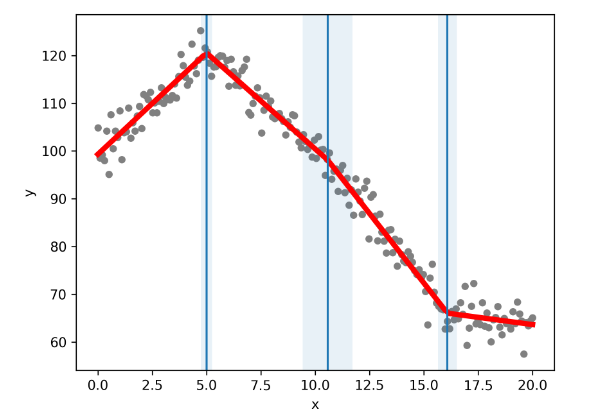
\includegraphics[width=0.6\textwidth]{figures/lin_growth.png}
        \caption{Piecewise linear growth curve}
        \label{fig:piecewise_linear}
    \end{figure}

    \item \textbf{Logistic growth:} 
    $$g(t) = \frac{C(t)}{1 + \exp(-(k + a(t)^T \delta)(t-(m + a(t)^T\gamma)))}$$

    It handles non-linear growth with saturation, i.e., the initial stage of growth is
    approximately exponential (geometric), then as saturation begins, the growth slows to 
    linear (arithmetic) and at maturity, the growth stops.

    \begin{figure}[H]
        \centering
        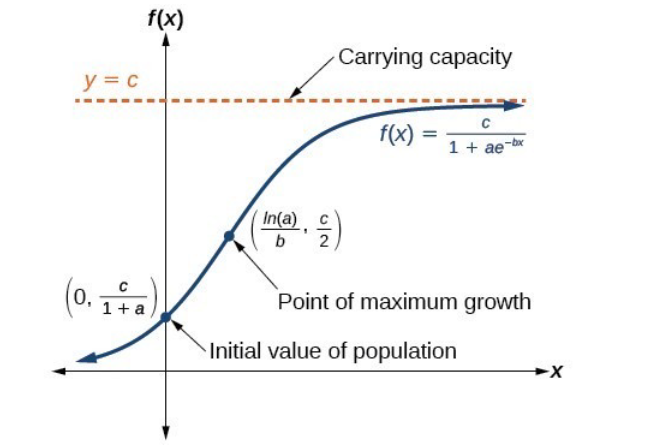
\includegraphics[width=0.6\textwidth]{figures/log_growth.png}
        \caption{Logistic growth curve}
        \label{fig:logistic_growth}
    \end{figure}

\end{itemize}

Notice that the term $a(t)$ is a binary vector that indicates the presence of changepoints
at time $t$. The term $C(t)$ is the carrying capacity of the growth curve, and it avoids
the infinite or negative growth of the logistic curve. 

\subsubsection{Seasonal function}

This function captures periodic changes in the value of the time series. It relies on
Fourier series to provide a malleable model of periodic effects. The seasonal component
$s(t)$ provides adaptability to the model b allowing periodic changes based on sub-daily,
daily, weekly, and yearly patterns.\\

The seasonal function is defined as:

$$s(t) = \sum_{n=1}^N \left(a_n \cos\left( \frac{2 \pi nt}{P} \right) + b_n \sin\left( \frac{2 \pi nt}{P} \right) \right)$$

where $N$ is the number of Fourier terms, $P$ is the period of the seasonality, and $a_n$
and $b_n$ are the Fourier coefficients.\\

Multiple seasonalities can be modeled with Fourier series with a smoothing prior and 
a low-pass filter. Notice that truncating the series at $N$ applies a low-pass filter
to the seasonality. So, along with increasing the risk of overfitting, increasing $N$
allows for fitting seasonal patterns that change more rapidly.\\

Note that we can write the seasonal function as a matrix multiplication:

$$s(t) = X(t) \cdot \beta$$

where $X(t)$ is the matrix of Fourier terms and $\beta$ is the vector of Fourier coefficients.
Also, $\beta \sim N(0, \sigma^2)$ as a prior. The choice of $N$ is a hyperparameter that 
can be tuned using indicators like the AIC.

\subsubsection{Holiday function}

This function adds peaks and drops that can be explained by holidays. It can account for 
holidays with dates that changes year to year, like Easter, Thanksgiving, etc.\\

Holidays are modeled as independent dummy external regressors allowing the inclusion 
of a window of days around the holidays to model their effects. The holiday function
$h(t)$ is defined as:

$$h(t) = \sum_{j=1}^J k_j \cdot I(t \in S_j)$$

where $J$ is the number of holidays, $k_j$ is the effect of holiday $j$, and $I(t \in S_j)$
is an indicator function that is 1 if $t$ is in the window of holiday $j$ and 0 otherwise.
We can rewrite the holiday function as a matrix multiplication:

$$h(t) = Z(t) \cdot \kappa, \quad Z(t) = \begin{bmatrix} I(t \in S_1) \\ I(t \in S_2) \\ \vdots \\ I(t \in S_J) \end{bmatrix}$$

where $Z(t)$ is the matrix of holiday indicators and $\kappa$ is the vector of holiday effects.
As with seasonalities, Prophet uses a prior $\kappa \sim N(0, \sigma^2)$.

\subsubsection{Additional regressors}

It is also posible to add exogenous variables, i.e., additional regressors. Prophet 
provides a more general interface for defining extra linear regressors and does not 
require that the regressor be a binary indicator. Another time series could be used 
as a regressor, although its future values would have to be known to make forecasts.\\

Additional regressors are a generalization of the holidays and events, which are
binary indicators.

\subsection{Where Prophet shines}

Prophet is optimized for the business forecast tasks at Meta, which typically have any
of the following characteristics:

\begin{itemize}
    \item Hourly, daily or weekly observations with at least a few months (preferably a year)
    of history.

    \item Strong multiple "human-scale" seasonalities: day of week and time of year.
    
    \item Important holidays that occur at irregular intervals that are known in advance
    (e.g., the Super Bowl).

    \item A reasonable number of missing observations or large outliers.
    
    \item Historical trend changes, for instance due to product launches or logging changes.
    
    \item Trends that are non-linear growth curves, where a trend hits a natural limit or
    saturates.
\end{itemize}

\section{Deep learning for time series forecasting}

For four decades, the "mantra" in applied forecasting has been "simple models outperform
complex models", influenced largely by the results of the Makridakis series forecasting
competition. This, until the most recent M-competitions, where every top solution
\textbf{relied on Machine Learning}.\\

There were some serious challenges faced by standard existing models. Most methods were
designed to forecasting individual series or small groups. From this, new problems emerged:
\begin{itemize}
    \item Forecasting \textbf{many} individual or grouped time series.
    
    \item Trying to learn a global model facing the difficulty of \textbf{dealing 
    with scale of different time-series} that would otherwise be related.
    
    \item Many classical models cannot \textbf{account for exogenous} or \textbf{multivariate
    inputs}.

    \item \textbf{Cold start problem} for new items to be included in the forecast.
\end{itemize}

This provided a set of goals for novel models. In general, they would need to have the 
ability to \textbf{learn} and \textbf{generalize from similar series}, that provides the
ability to learn more complex models without overfitting; and the ability to \textbf{estimate
the probability distribution} of a time series future, given its past (\textbf{probabilistic
forecasting}).

\subsection{DeepAR}

One of the first solutions to these problems was the \textbf{DeepAR} model, developed by
Amazon. It is a forecasting model based on \textbf{Autoregressive RNNs}, which learns
a \textbf{global} model from historical data \textbf{of all time series} in all 
datasets.\\

DeepAR is the first succesful model to \textbf{combine Deep Learning} with traditional
\textbf{Probabilistic Forecasting}. Its main advantages are:

\begin{itemize}
    \item \textbf{Multiple time-series support:} the model is trained on multiple time 
    series, learning global characteristics that further enhance forecasting accuracy.

    \item \textbf{Extra covariates:} DeepAR allows extra features (covariates). For instance,
    if your task is temperature forecasting, you can include humidity-level, air-pressure, etc.

    \item \textbf{Probabilistic output:} instead of making a single prediction, the model
    leverages Monte Carlo samples to output prediction intervals.

    \item \textbf{"Cold" forecast:} by learning from thousands of time series that 
    potentially share a few similarities, DeepAR can provide forecasts for time-series
    that have little to no historical data.
\end{itemize}

\subsection{DeepAR under the hood}

DeepAR is a \textbf{sequence-to-sequence} model. It uses \textbf{LSTM} networks to 
create probabilistic outputs. Note that LSTMs are used in numerous time series 
forecasting model architectures:
\begin{itemize}
    \item Multi-stacked LSTMs.
    \item LSTMs with CNNs
    \item LSTMs in encoder-decoder architectures
    \item Etc...
\end{itemize}

Contrary to the previous models, DeepAR uses LSTMs a but different: instead of using them
to calculate predictions directly, DeepAR \textbf{leverages LSTMs to predict all parameters
of a probability distribution} for the next time point. For instance, DeepAR estimates
the $\theta = (\mu, \sigma)$ of a Gaussian distribution.

\begin{figure}[H]
    \centering
    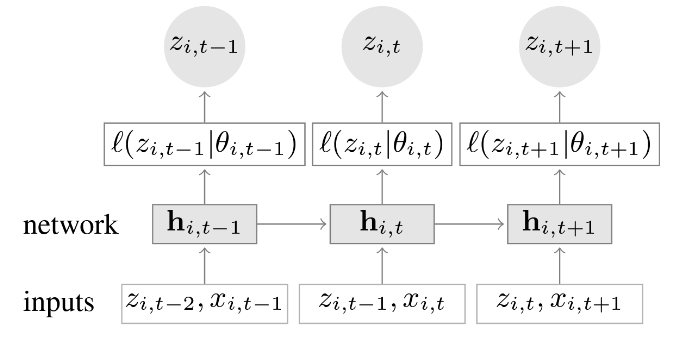
\includegraphics[width=0.6\textwidth]{figures/lstm_deepar.png}
    \caption{Simple diagram of LSTMs in DeepAR}
    \label{fig:lstm_deepar}    
\end{figure}

Then, based on the result of the LSTM, DeepAR uses \textbf{two dense layers to
derive the parameters of the distribution}. The first dense layer is used to calculate
the mean $\mu$ of the distribution, and the second dense layer is used to calculate the 
standard deviation $\sigma$ of the distribution.

\begin{figure}[H]
    \centering
    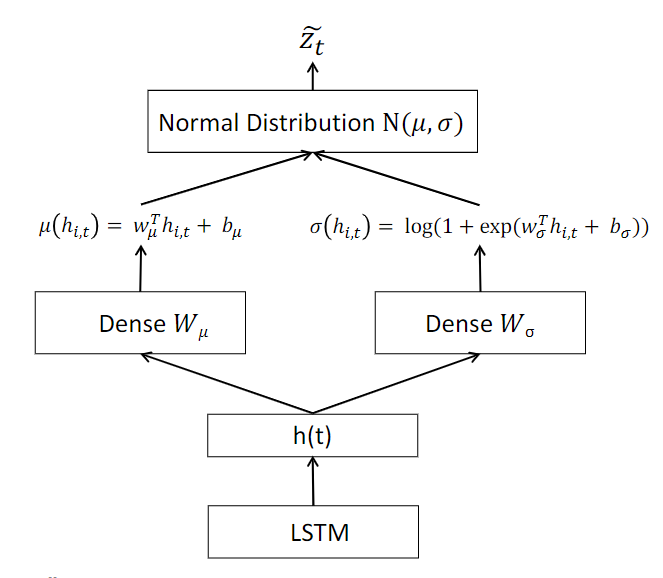
\includegraphics[width=0.5\textwidth]{figures/deepar.png}
    \caption{DeepAR architecture}
    \label{fig:deepar}
\end{figure}

DeepAR in various tests \textbf{outperformed traditional statistical methods} such 
as ARIMA. Also, the great advantage of DeepAR over those models is that \textbf{it 
does not require extra featuring preprocessing} (e.g., making the time series stationary
first). This model os \textbf{prevalent in production}: it is part of Amazon's GluonTS
toolkit for timeseries forecasting and it can be trained on Amazon SageMaker.\\

There are various other models like the following:

\begin{figure}[H]
    \centering
    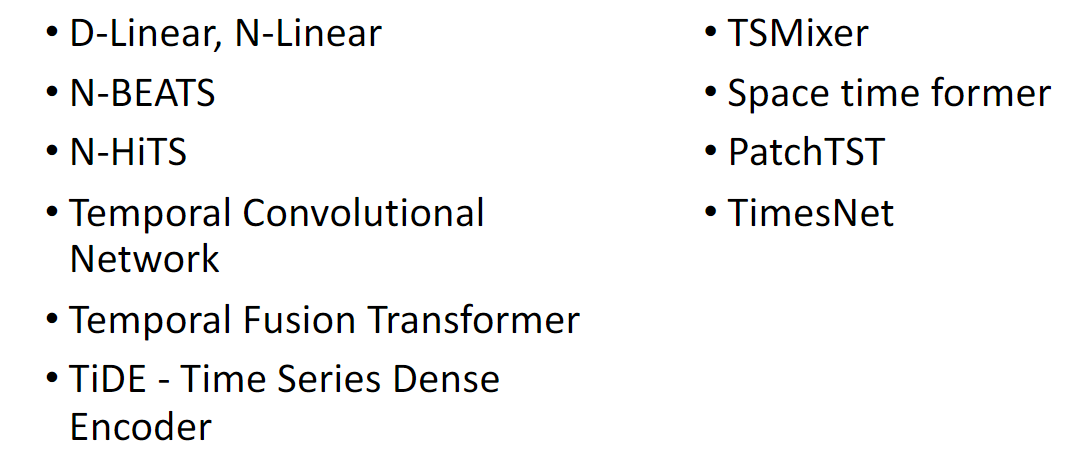
\includegraphics[width=0.8\textwidth]{figures/other_models.png}
    \caption{Deep learning models for time series forecasting}
    \label{fig:deep_learning_models}
\end{figure}

\subsection{Trade-offs}

Deep learning models have some trade-offs that need to be considered. For instance,
they are \textbf{computationally expensive} and \textbf{require large amounts of data}.
Also, they are \textbf{black-box models}, which means that they are difficult to interpret
and understand.

\begin{figure}[H]
    \centering
    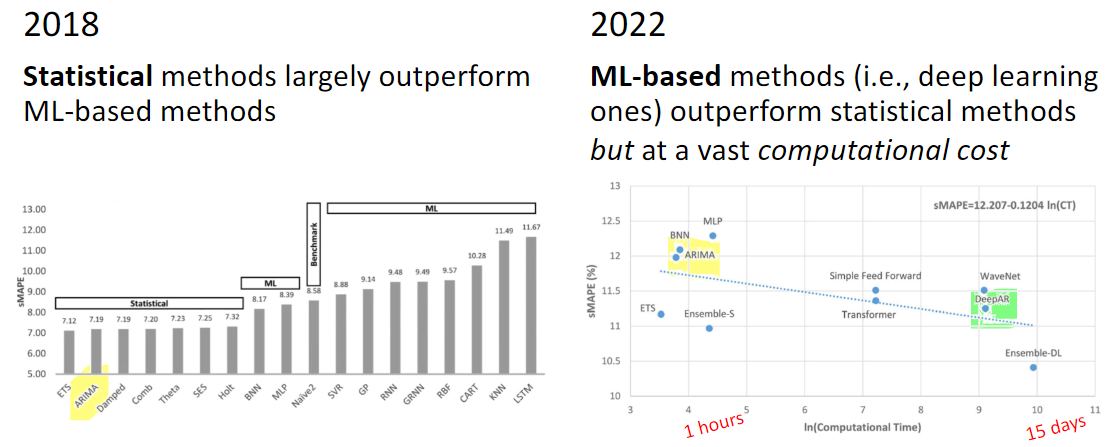
\includegraphics[width=1\textwidth]{figures/trade_offs.png}
    \caption{Trade-offs of deep learning models}
    \label{fig:trade_offs}
\end{figure}
